\documentclass{article}
\usepackage{amssymb} % Required for math symbols
\usepackage{graphicx} % Required for inserting images
\usepackage[hidelinks]{hyperref}
\usepackage{float}

\usepackage[utf8]{inputenc}
\usepackage{amsmath}
\usepackage[a4paper, total={6in, 10in}]{geometry}
\usepackage{listings}
\usepackage{xcolor}

\definecolor{codegray}{rgb}{0.5,0.5,0.5}
\definecolor{codepurple}{rgb}{0.58,0,0.82}
\definecolor{backcolour}{rgb}{0.95,0.95,0.92}

\lstdefinestyle{cppstyle}{
    backgroundcolor=\color{backcolour},   
    commentstyle=\color{codegray}\ttfamily,
    keywordstyle=\color{blue}\bfseries,
    numberstyle=\tiny\color{gray},
    stringstyle=\color{codepurple},
    basicstyle=\ttfamily\footnotesize,
    breaklines=true,
    captionpos=b,
    keepspaces=true,
    numbers=left,
    numbersep=5pt,
    showspaces=false,
    showstringspaces=false,
    showtabs=false,
    tabsize=2,
    language=C++
}

\title{Laboratorio 2 - Sensores y Actuadores}
\author{jeremy.matos@utec.edu.pe, luis.gutierrez@utec.edu.pe, plinio.avendano@utec.edu.pe}
\date{Abril 2025}

\begin{document}

\maketitle

\newpage
\tableofcontents
\newpage

\section{Introducción}

\subsection{Objetivo General}

Diseñar, implementar y documentar sistemas completos de sensor-actuador, con el propósito de entender a cabalidad su funcionamiento.

\subsection{Objetivos Específicos}

\begin{itemize}
    \item Modelar y simular la activación directa de un motor DC con Arduino, determinando límites seguros de corriente y tensión, y analizando cómo la entrada analógica del potenciómetro condiciona el encendido del motor.
    \item Diseñar circuitos de conmutación basados en relés para cargas inductivas, aplicando diodos fly-back y fuentes externas para aislar la etapa de potencia; luego contrastar su desempeño y versatilidad con las soluciones basadas en drivers.
    \item Desarrollar sistemas utilitarios empleando todos los conceptos aprendidos, plasmando en soluciones prototiparias problemas de la vida real como un sistema de riego inteligente.
\end{itemize}

\newpage

\section{Marco teórico}

\section{Estado del Arte}

Las arquitecturas modernas de sensor–actuador para sistemas IoT parten de redes inalámbricas de muy bajo consumo que recogen el estado del entorno y disparan actuadores distribuidos. Un referente es SM-Light, que demostró cómo un WSN de alumbrado público reduce un 40\% la energía al activar luminarias mediante nodos ultra-low-power y pasarelas multihop. \cite{karapetyan2020smlight}

En la misma línea, Sajini y Pushpa integran sensores ultrasónicos y visión por computador sobre Raspberry Pi para asistencia a invidentes, destacando la fiabilidad de lazo cerrado entre sensado e iluminación/buzzers accionados desde la nube. \cite{sajini2023proximity}

Estos trabajos posicionan al microcontrolador como orquestador de la lógica, mientras que el subsistema de potencia se delega a drivers o relés aislados; un requisito que nuestra práctica de laboratorio satisface con módulos L298N y relés de 5V.

En cuánto al control de motores DC, la literatura converge en usar puentes H acompañados de modulación PWM para gobernar velocidad y reversa. Tesfaye y Liu describen un esquema con Arduino Uno que logra ±5 \% de error en velocidad combinando PWM de 490 Hz con lógica L293D/L298N, validando su idoneidad para educación y robótica ligera. \cite{kaffale2025dcmotor}

Para tareas de conmutación on/off de cargas donde no se requiere inversión de sentido, la comunidad opta por relés electromecánicos o por relés de estado sólido (SSR) que aíslan la MCU mediante optoacopladores. Medina et al. presentan un SSR de duty-cycle variable gobernado vía Wi-Fi que maneja 120 V / 10 A y reporta tensión, corriente y factor de potencia al usuario, ilustrando la tendencia a integrar sensado de potencia en el propio actuador. \cite{medina2024ssr} 

Plasmando estos conceptos a sistemas utilitarios en vida real, en aplicaciones agrícolas, los sistemas de riego inteligente accionan bombas de agua a través de relés de 5 V controlados por NodeMCU, demostrando ahorros de hasta 25 \% en consumo hídrico y trazabilidad vía Blynk o ThingSpeak. \cite{muthekar2024smartirr}

En síntesis, el estado del arte converge en tres principios que se reflejan en nuestra guía de laboratorio:

Separar la lógica de control del plano de potencia mediante drivers o relés con aislamiento adecuado.

Utilizar PWM para regular energía —velocidad en motores o intensidad luminosa— con microcontroladores de propósito general.

Conectar los actuadores a plataformas IoT para monitorizar variables eléctricas y ambientales en tiempo real, habilitando optimización energética y mantenimiento predictivo. Estos lineamientos, respaldados por la literatura citada, fundamentan la elección de los módulos relé y L298N, así como la inclusión de prácticas de medición y protección (diodo) que el laboratorio exige implementar.


% file:///home/tenken/Downloads/30_ShodhKosh_RS_5111.pdf

% https://www.etasr.com/index.php/ETASR/article/view/6410

% https://users.cecs.anu.edu.au/~sid.chau/papers/TOSN-smlight.pdf

% https://www.semanticscholar.org/paper/Innovative-IoT-Smart-Lock-System:-Enhancing-with-Zainuddin-Rahman/563edb5ed5795c9bb35eefc69aa010c9f7c60157

\section{Metodología}

\subsection{SENSORES - Sensor de luz ambiental}

% DONE: Simulacion

En esta experiencia de laboratorio, se desarrollará un sistema de medición ambiental utilizando los siguientes componentes: 
\begin{itemize}
    \item 1 LDR (sensor de luz)
    \item Diodos LED
    \item Buzzer (alarma)
    \item Botón o switch
\end{itemize}

El objetivo es implementar un sistema que permita medir la cantidad de luz en un ambiente determinado, el cual complementará un sistema de cámaras de seguridad y un control inteligente de luminarias. El sistema debe cumplir con las siguientes funciones:
\begin{enumerate}
    \item Si el nivel de iluminación es bajo, las luminarias de la habitación deben encenderse, representado por el encendido de un LED rojo.
    \item Si el nivel de iluminación es alto, las luminarias deben permanecer apagadas, representado por el LED rojo apagado.
    \item Las cámaras de seguridad deben estar en funcionamiento en todo momento, lo cual se representa mediante el encendido de un LED azul.
    \item En caso de que no se detecte energía eléctrica para el sistema de cámaras (entrada digital detecta GND), el sistema debe encender y apagar el LED azul de manera intermitente, además de activar un buzzer que representa una alarma de error. Esto puede simularse utilizando un botón, un switch o una desconexión de cable.
\end{enumerate}

La implementación se realizó en la plataforma Tinkercad, utilizando un Arduino UNO. La conexión de los componentes se puede observar en la Figura \ref{fig:luz_ambiental}. El sensor LDR se conectó a una entrada analógica (A0), mientras que los LEDs y el buzzer se conectaron a salidas digitales. Un botón se empleó como entrada digital para simular la presencia o ausencia de energía del sistema de cámaras.

\begin{figure}[H]
    \centering
    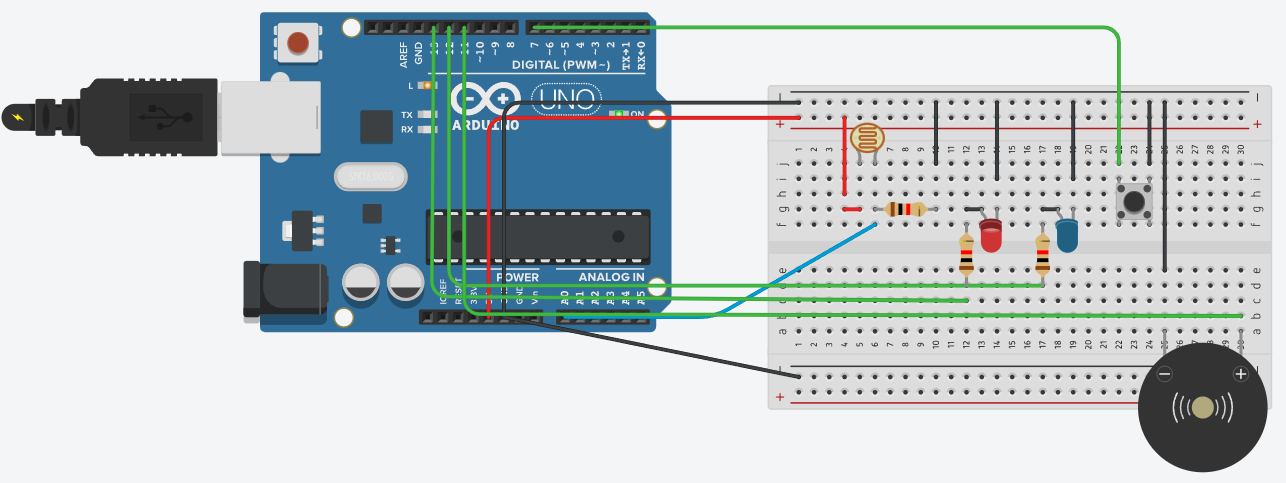
\includegraphics[width=0.85\textwidth]{./img/ckpt_1.png}
    \caption{Simulación Tinkercad Sensor de luz ambiental}
    \label{fig:luz_ambiental}
\end{figure}

En el código (Código \ref{code:sensor_ambiental}), se define un umbral de luminosidad para distinguir entre un ambiente claro u oscuro. Si el valor leído del LDR es menor que este umbral, se activa el LED rojo. Por otro lado, si el botón indica que hay energía (estado HIGH), el LED azul permanece encendido de forma constante. En caso contrario (estado LOW), el sistema simula una falla eléctrica encendiendo el buzzer y haciendo parpadear el LED azul.

\begin{lstlisting}[style=cppstyle, caption={Código en C++ para el sensor ambiental.}, label={code:sensor_ambiental}]
int LDR_pin = A0;
int ROJO_pin = 13;
int AZUL_pin = 12;
int BUZZER_pin = 11;
int BUTTON_pin = 7;
int luz, estadoBoton;
const int umbral = 500;  // Ajustarlo

void setup() {
    pinMode(ROJO_pin, OUTPUT); pinMode(AZUL_pin, OUTPUT);
    pinMode(BUZZER_pin, OUTPUT);
    pinMode(BUTTON_pin, INPUT_PULLUP);
    Serial.begin(9600);
}

void loop() {
    luz = analogRead(LDR_pin);
    estadoBoton = digitalRead(BUTTON_pin);
    Serial.println("Luz: " + String(luz) + " - " + String(umbral));
    
    if (luz < umbral) digitalWrite(ROJO_pin, HIGH);
    else digitalWrite(ROJO_pin, LOW);
    
    if (estadoBoton == HIGH) {
        digitalWrite(AZUL_pin, HIGH);
        digitalWrite(BUZZER_pin, LOW);
    } else {
        digitalWrite(BUZZER_pin, HIGH);
        digitalWrite(AZUL_pin, HIGH); delay(300);
        digitalWrite(AZUL_pin, LOW); delay(300);
    }
    delay(1000);
}    
\end{lstlisting}

\begin{figure}[H]
    \centering
    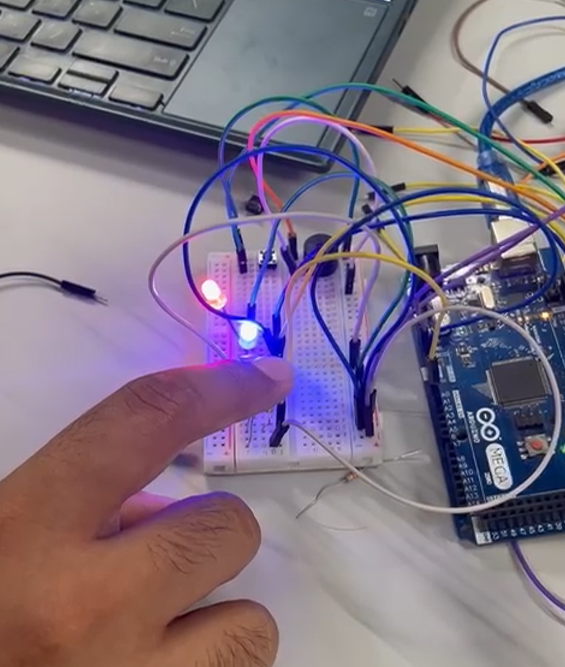
\includegraphics[width=0.85\textwidth]{img/sensores_chkp_2.png}
    \caption{Simulación Tinkercad Sensor de luz ambiental}
    \label{fig:luz_ambiental}
\end{figure}

\begin{figure}[H]
    \centering
    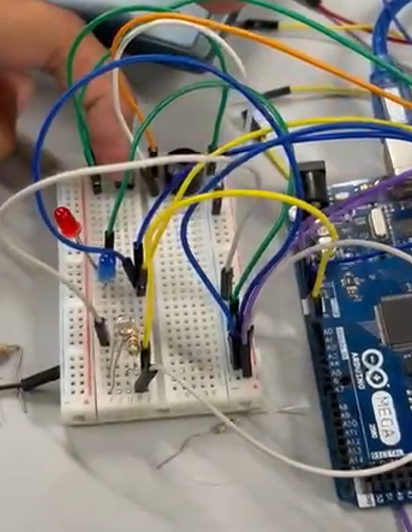
\includegraphics[width=0.85\textwidth]{img/sensores_chkp_2_1.png}
    \caption{Simulación Tinkercad Sensor de luz ambiental}
    \label{fig:luz_ambiental}
\end{figure}

% TODO: foto de la implementacion presencial en el laboratorio

\subsection{SENSORES - Cerradura inteligente}

% TODO: Diagrama de flujo
% DONE: Simulacion
En esta experiencia de laboratorio, se desarrollará un sistema de seguridad para el control de acceso de personas a un área restringida. Para ello, se utilizarán los siguientes componentes: 

\begin{itemize}
    \item 01 sensor de proximidad.
    \item 01 teclado matricial.
    \item 01 LCD 2x16.
    \item Diodos LED.
    \item Resistencias variadas.
    \item Jumpers.
\end{itemize}

La solución final se puede ver en la Figura \ref{fig:cerradura_smart}. En las siguientes subsecciones se desglosarán las diferentes funcionalidades del sistema.

\begin{figure}[H]
    \centering
    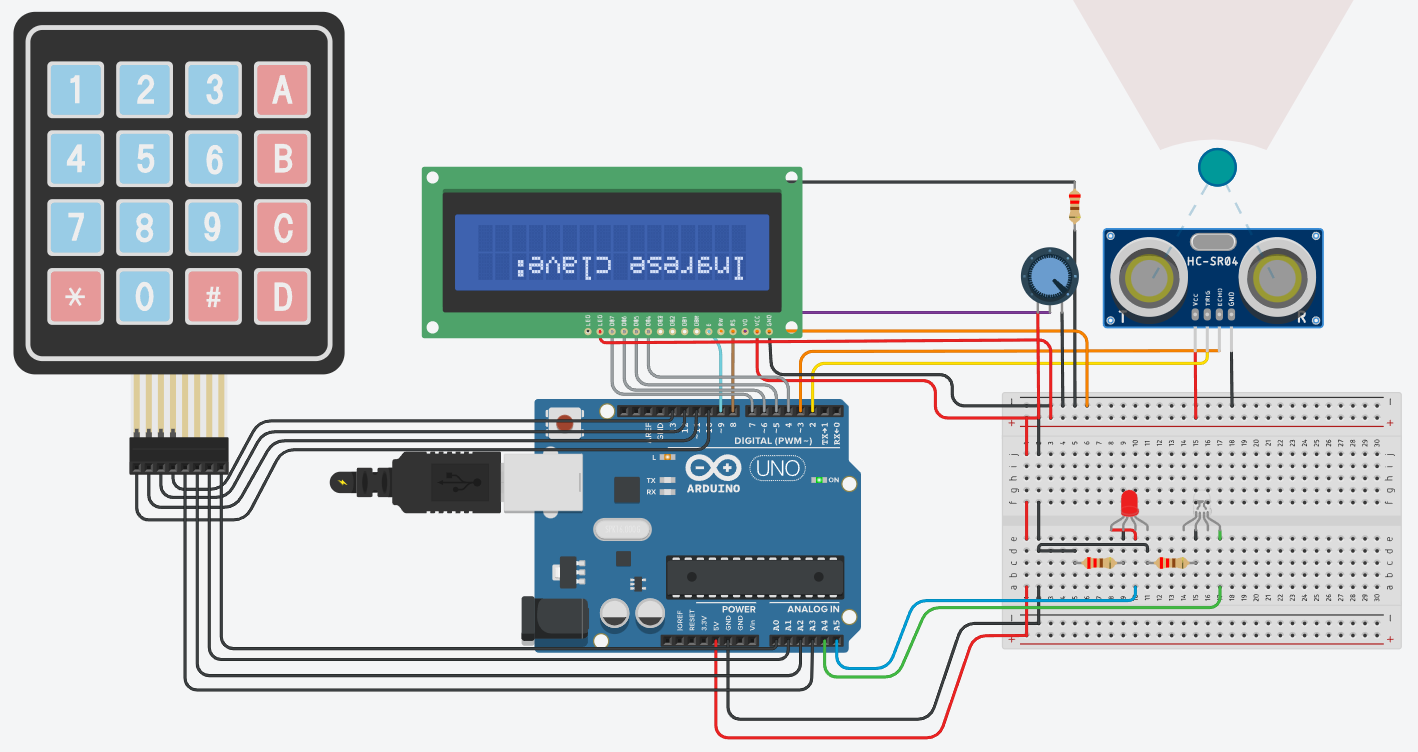
\includegraphics[width=0.85\textwidth]{./img/ckpt_6.png}
    \caption{Simulación Tinkercad Resultado final del sistema de cerradura inteligente}
    \label{fig:cerradura_smart}
\end{figure}

% TODO: foto de la implementacion presencial en el laboratorio

\subsubsection{Presencia de la persona}

\subsubsection{Mensaje en LCD}

\subsubsection{Autenticación}

\subsubsection{Ahorro Energético (Standby)}

\subsection{SENSORES - Sistema de control de aforo}

% DONE: Simulacion

\begin{figure}[H]
    \centering
    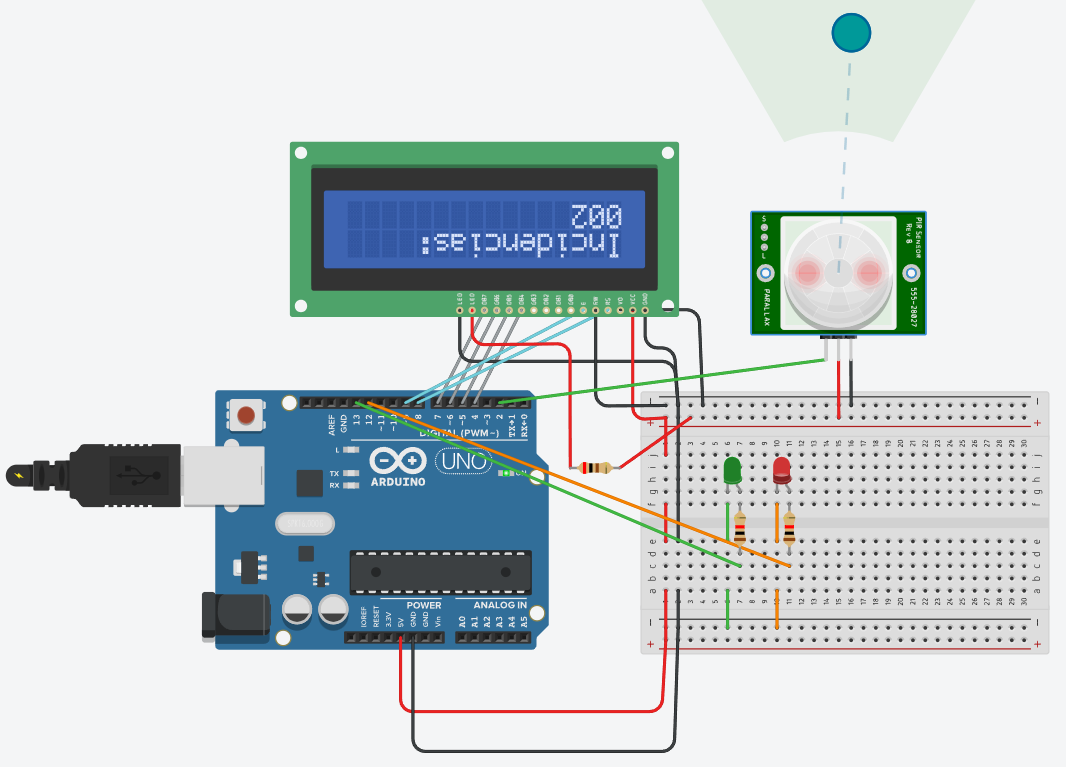
\includegraphics[width=0.85\textwidth]{./img/ckpt_9.png}
    \caption{Simulación Tinkercad Resultado final del sistema de control de aforo}
    \label{fig:control_aforo}
\end{figure}

\begin{lstlisting}[style=cppstyle, caption={Código en C++ para el sistema de control de aforo.}, label={code:sensor_ambiental}]
#include <LiquidCrystal.h>

// Configuracion del LCD
LiquidCrystal lcd(8, 9, 4, 5, 6, 7);
const int PIRPin = 2;
const int LEDGreen = 13;
const int LEDRed = 12;

// Variable to store the number of incidents
int incidentCount = 0;

void setup() {
    Serial.begin(9600);
    
    lcd.begin(16, 2);
    lcd.clear();
    pinMode(PIRPin, INPUT);
    pinMode(LEDGreen, OUTPUT);
    pinMode(LEDRed, OUTPUT);
}

void loop() {
    int value = digitalRead(PIRPin);
    Serial.println(value);

    if (value == LOW) {
    // No movement detected, indicating the rest mode
    digitalWrite(LEDGreen, HIGH);   // Green LED blink (indicates idle state)
    delay(200);
    digitalWrite(LEDGreen, LOW);
    delay(200);
    
    // Display "RESTING" on LCD when no movement detected
    lcd.clear();
    lcd.setCursor(0, 0);
    lcd.print("Modo de Reposo");
    } else {
    // Movement detected, indicating the active state
    digitalWrite(LEDGreen, LOW);    // Turn off the green LED
    digitalWrite(LEDRed, HIGH);     // Turn on the red LED

    // Increment incident count when movement is detected
    incidentCount++;

    // Display incident count on LCD
    lcd.clear();
    lcd.setCursor(0, 0);
    lcd.print("Incidencias: ");
    lcd.setCursor(0, 1);
    lcd.print("00" + String(incidentCount));  // Assuming a 3-digit max count
    
    delay(2000); // Wait 2 seconds before checking again
    }
    
    delay(10);  // Small delay to stabilize the loop
}    
\end{lstlisting}
    
% TODO: foto de la implementacion presencial en el laboratorio
% TODO: diagrama de flujo
% TODO: diagrama de bloques
% ? TODO: checkpoint 5 y 6 son distintas simulaciones????


\subsection{ACTUADORES - Encendido de un Motor DC con Arduino}

% https://www.tinkercad.com/things/7Ta4Am5NLdF/editel?returnTo=%2Fdashboard%2Fdesigns%2Fcircuits&sharecode=ddM9-NkLnJGgaDXANovwieeo9xofWe2gha9ahUL3Y-o
\begin{figure}[H]
    \centering
    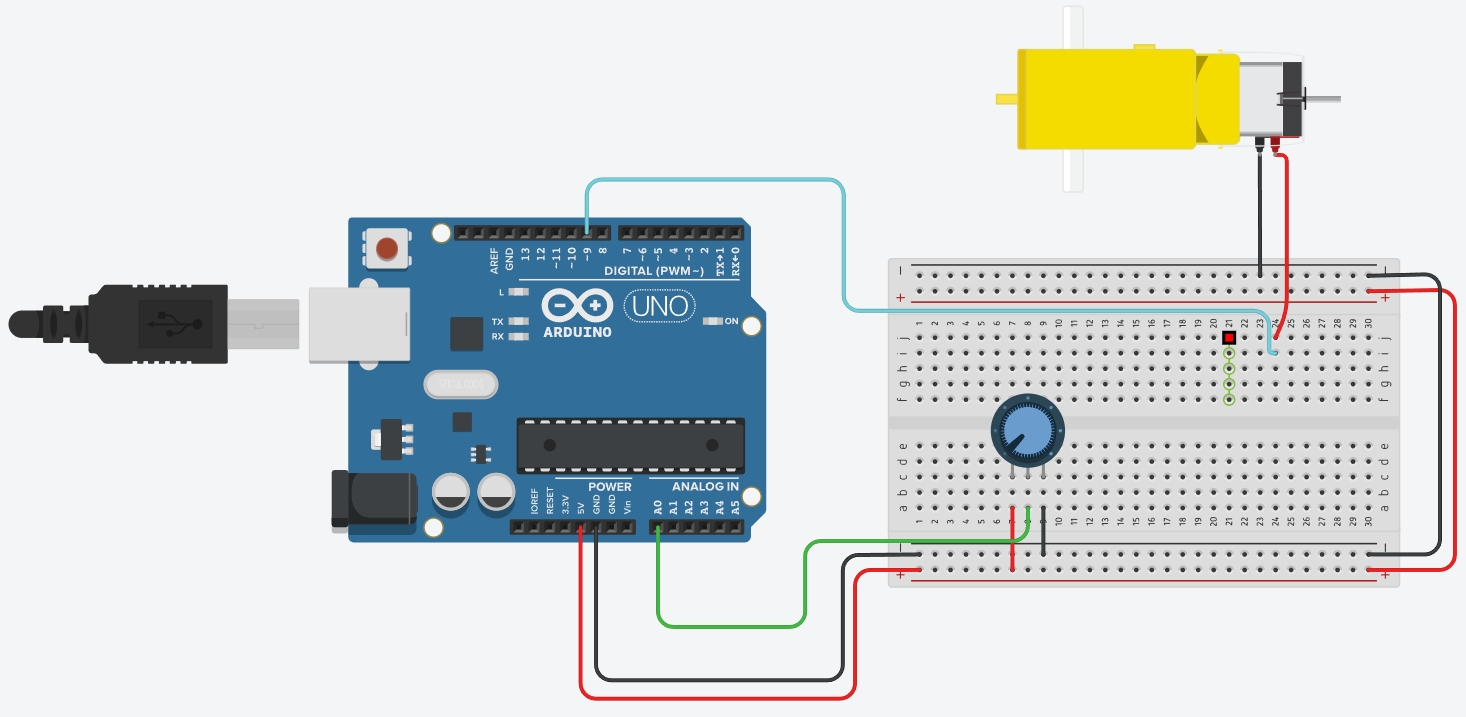
\includegraphics[width=0.85\textwidth]{./img/ckpt_encendido_motor.png}
    \caption{Simulación Tinkercad ...}
    \label{fig:encendido_motor}
\end{figure}

% TODO: simulacion
% TODO: diagrama de bloques
% TODO: respuesta a las preguntas

\begin{enumerate}
    \item ¿Cuál es la corriente que consume el motor durante su operación?
    \item Si usted quisiera regular la velocidad del motor, ¿qué añadiría a su esquema de conexión?
\end{enumerate}

\subsection{ACTUADORES - Control de un motor con Driver}

% https://www.tinkercad.com/things/6vFVydoth82/editel?returnTo=%2Fdashboard%2Fdesigns%2Fcircuits&sharecode=zm5Em3SqUbJ5xXMONP0ul2aEuINO3AnNjSSn-egeFUc

\begin{figure}[H]
    \centering
    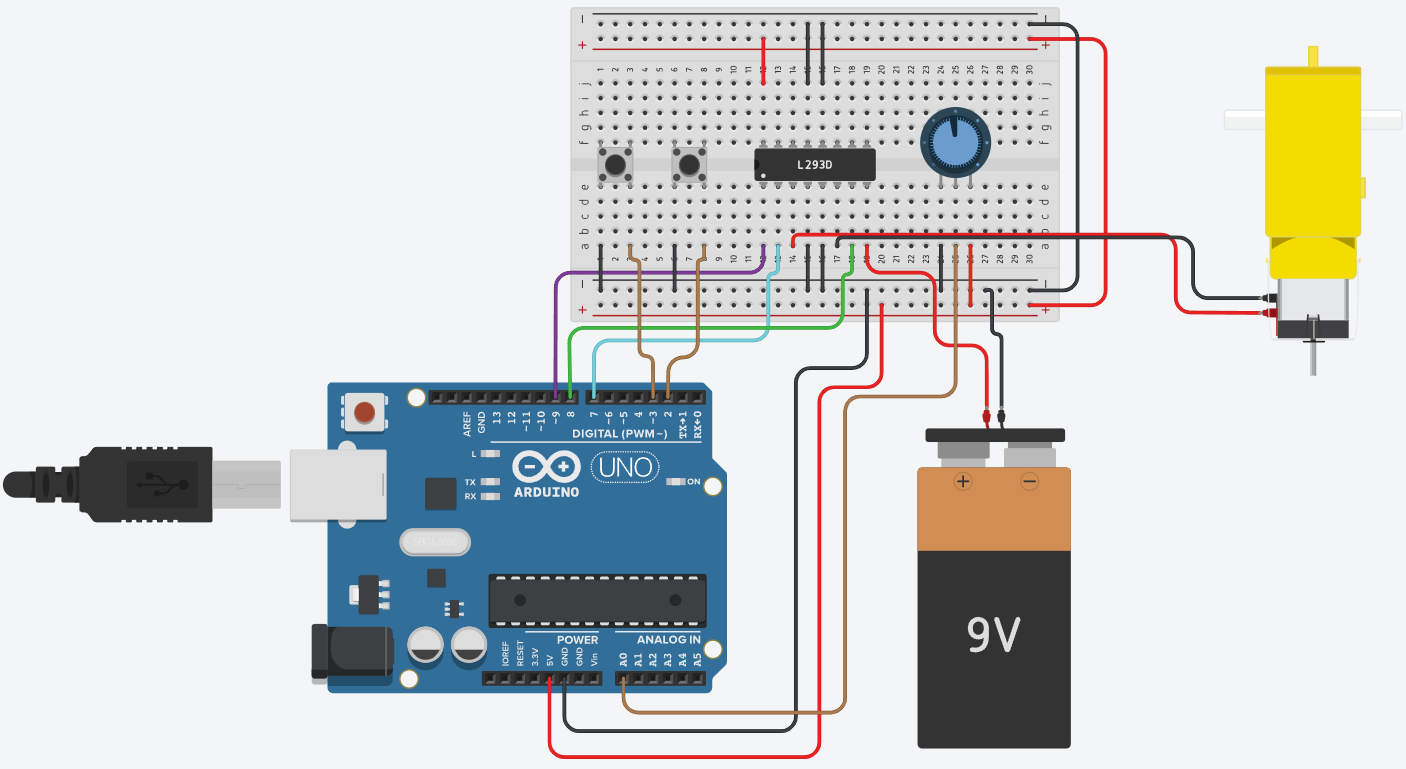
\includegraphics[width=0.85\textwidth]{./img/ckpt_motor_driver.png}
    \caption{Simulación Tinkercad ...}
    \label{fig:motor_driver}
\end{figure}

\begin{enumerate}
    \item ¿Cuál es la función del potenciómetro en este sistema de control de motor y cómo se
    relaciona con la velocidad de rotación?
    \item Explique por qué se requiere una fuente de alimentación externa para el motor en lugar de usar directamente la salida de 5V del Arduino.
    \item Describa el comportamiento esperado del motor cuando se presiona únicamente el botón
    derecho, el izquierdo, y cuando no se presiona ninguno. ¿Qué sucede si se presionan los dos?
\end{enumerate}

% TODO: simulacion
% TODO: diagrama de bloques
% TODO: respuesta a las preguntas


\subsection{ACTUADORES - Uso de Relé con Motor}

\begin{figure}[H]
    \centering
    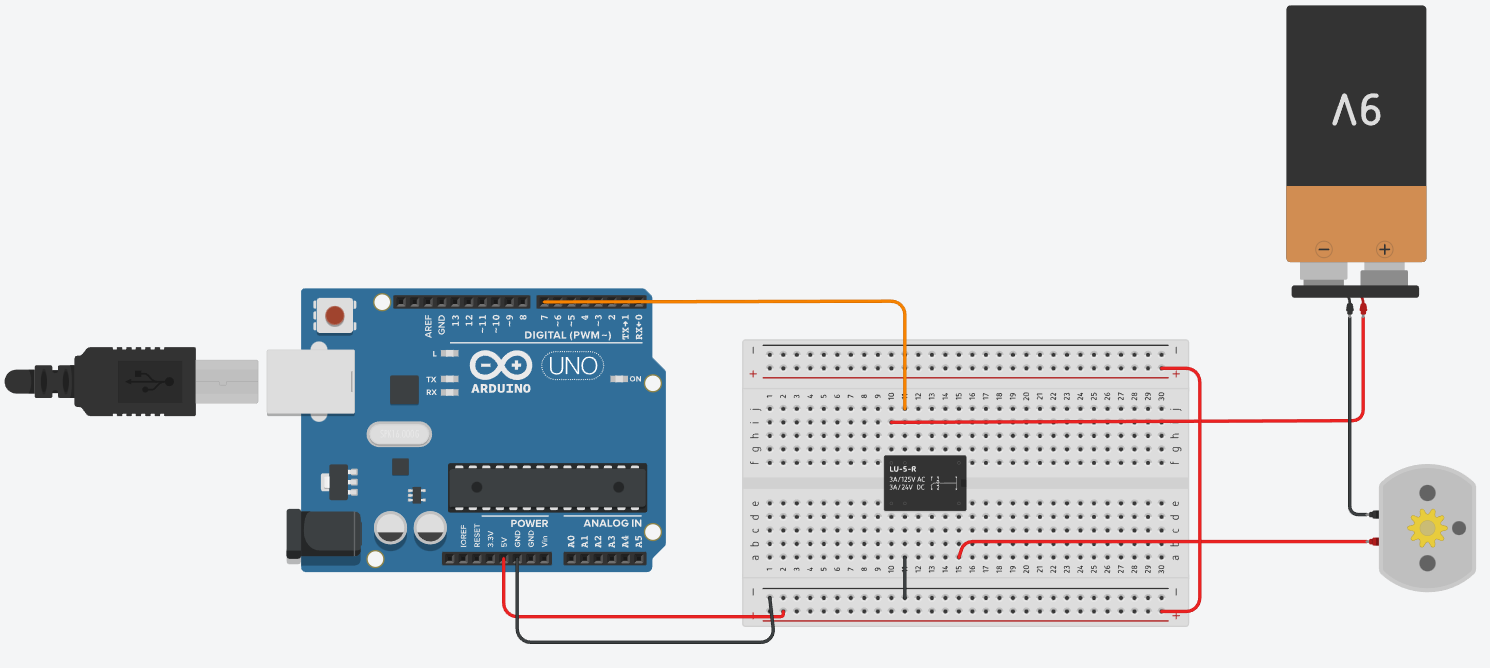
\includegraphics[width=0.85\textwidth]{./img/ckpt_rele_motor.png}
    \caption{Simulación Tinkercad}
    \label{fig:motor_driver}
\end{figure}

\begin{figure}[H]
    \centering
    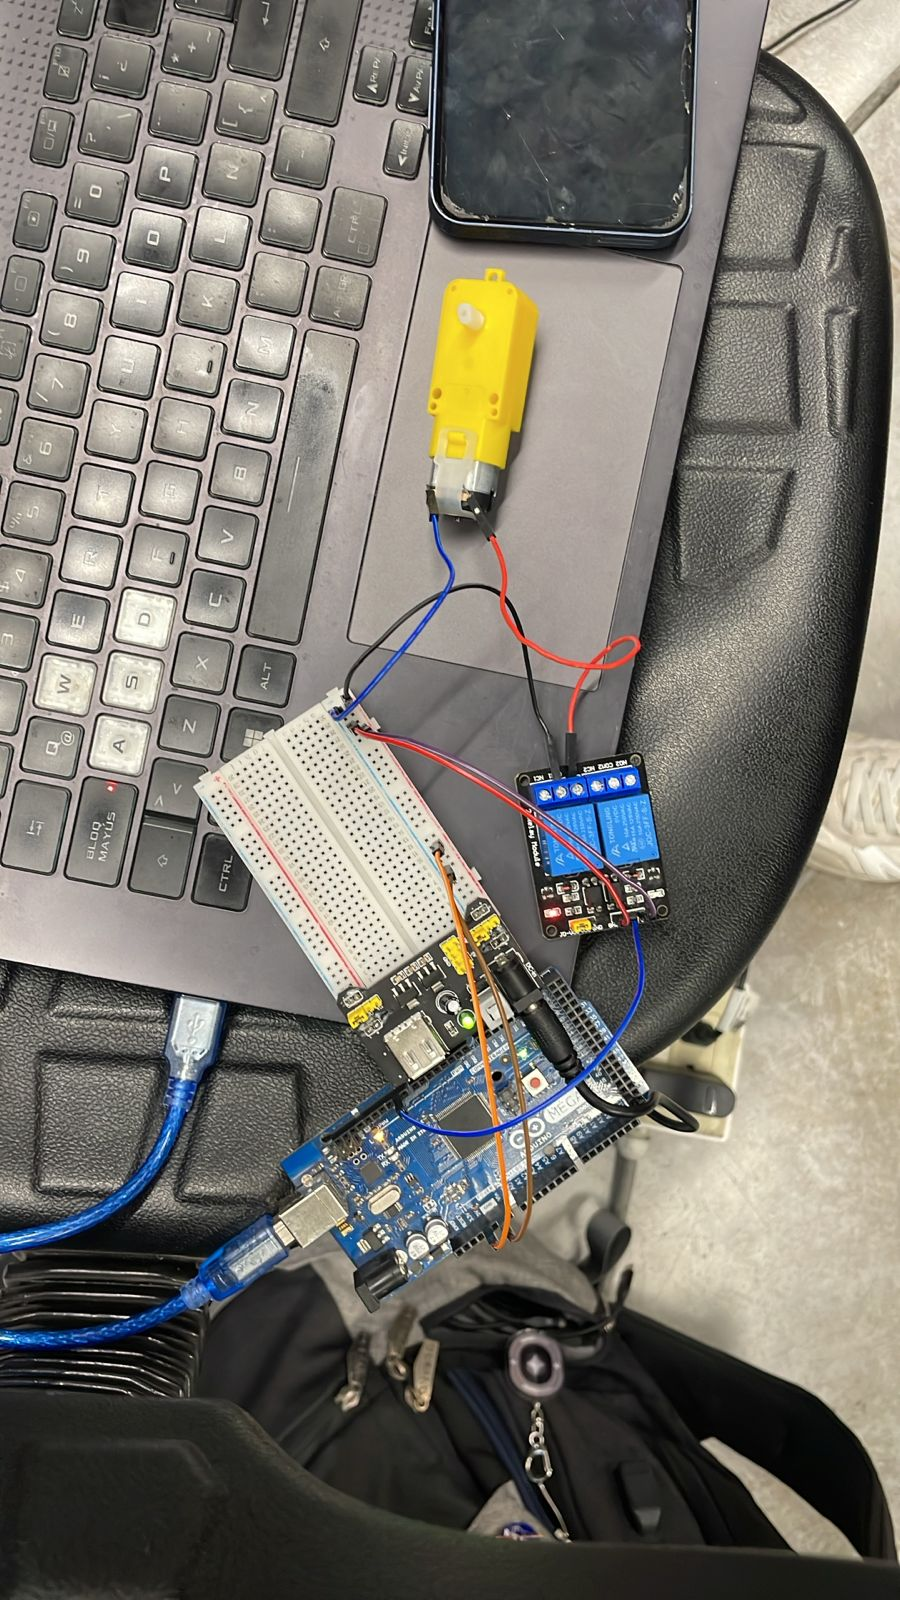
\includegraphics[width=0.85\textwidth]{./img/checkpoint_presencialrele.jpeg}
    \caption{Implementación del relé con motor}
    \label{fig:motor_driver}
\end{figure}

\begin{figure}[H]
    \centering
    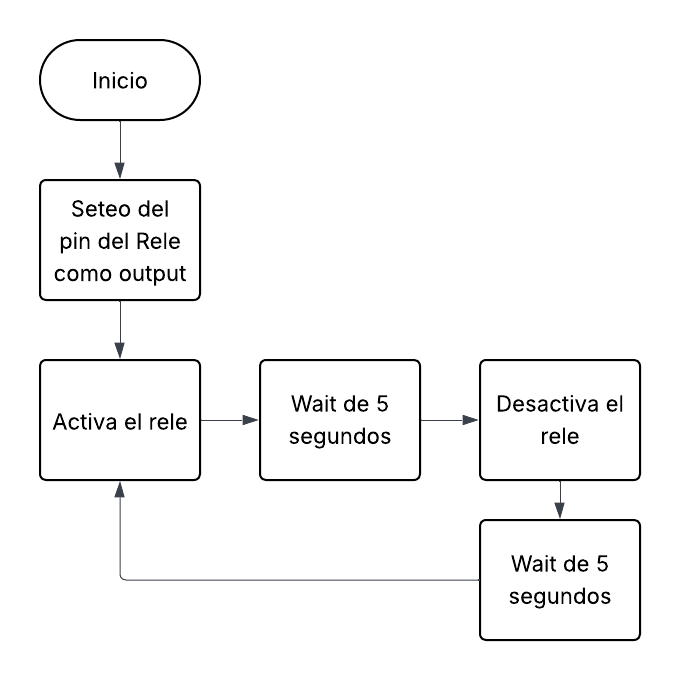
\includegraphics[width=0.85\textwidth]{./img/flujo_rele.png}
    \caption{Diagrama de flujo funcionamiento relé-motor}
    \label{fig:motor_driver}
\end{figure}

% DONE: simulacion
% DONE: foto de la implementacion presencial en el laboratorio
% DONE: diagrama de flujo
% TODO: diagrama de bloques

\subsection{ACTUADORES - Uso de Driver Puente H L298N con Motor}

\begin{enumerate}
    \item Prueba alimentar el módulo L298N directamente desde el pin de 5V del Arduino (en lugar de la fuente para protoboard). ¿Notas alguna diferencia en el rendimiento del motor? Justifica técnicamente tu observación.

    El rendimiento del motor decae, su movimiento se hace más lento y pierde fuerza. Esto es debido a que hemos cambiado de operar con una fuente de 9V a una de 5V.
        
    \item Restablezca la alimentación del motor. Modifica el circuito para invertir el sentido de giro automáticamente cada 3 segundos.

    Esto lo logramos invirtiendo los valores HIGH y LOW del in1 e in2.
    
    \item ¿Qué función cumple el pin ENA en el módulo L298N y por qué debe conectarse a un pin PWM del Arduino?

    Permitir regular la velocidad del motor, se conecta a un pin PWM debido a que estos permiten enviar una señal modulada que simula un voltaje medio variable. 
    
    \item ¿Qué sucede si se intercambian las conexiones de IN1 e IN2? ¿Cómo afecta esto a la dirección del giro del motor?

    Cambia la dirección del motor, de izquierda a derecha, respectivamente.
\end{enumerate}

\begin{figure}[H]
    \centering
    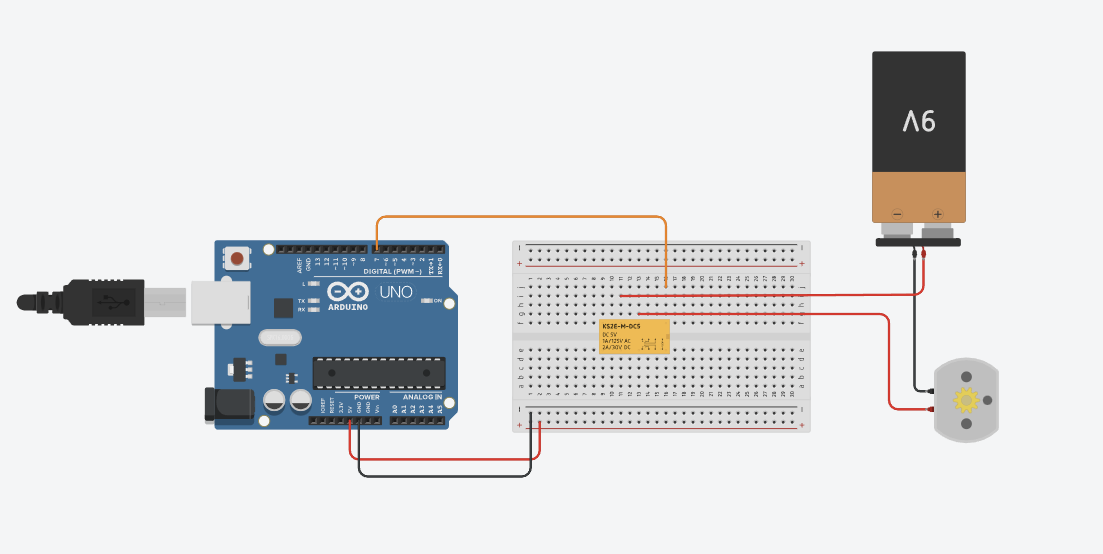
\includegraphics[width=0.85\textwidth]{./img/simulacion_puenteh.png}
    \caption{Simulación Tinkercad}
    \label{fig:motor_driver}
\end{figure}

\begin{figure}[H]
    \centering
    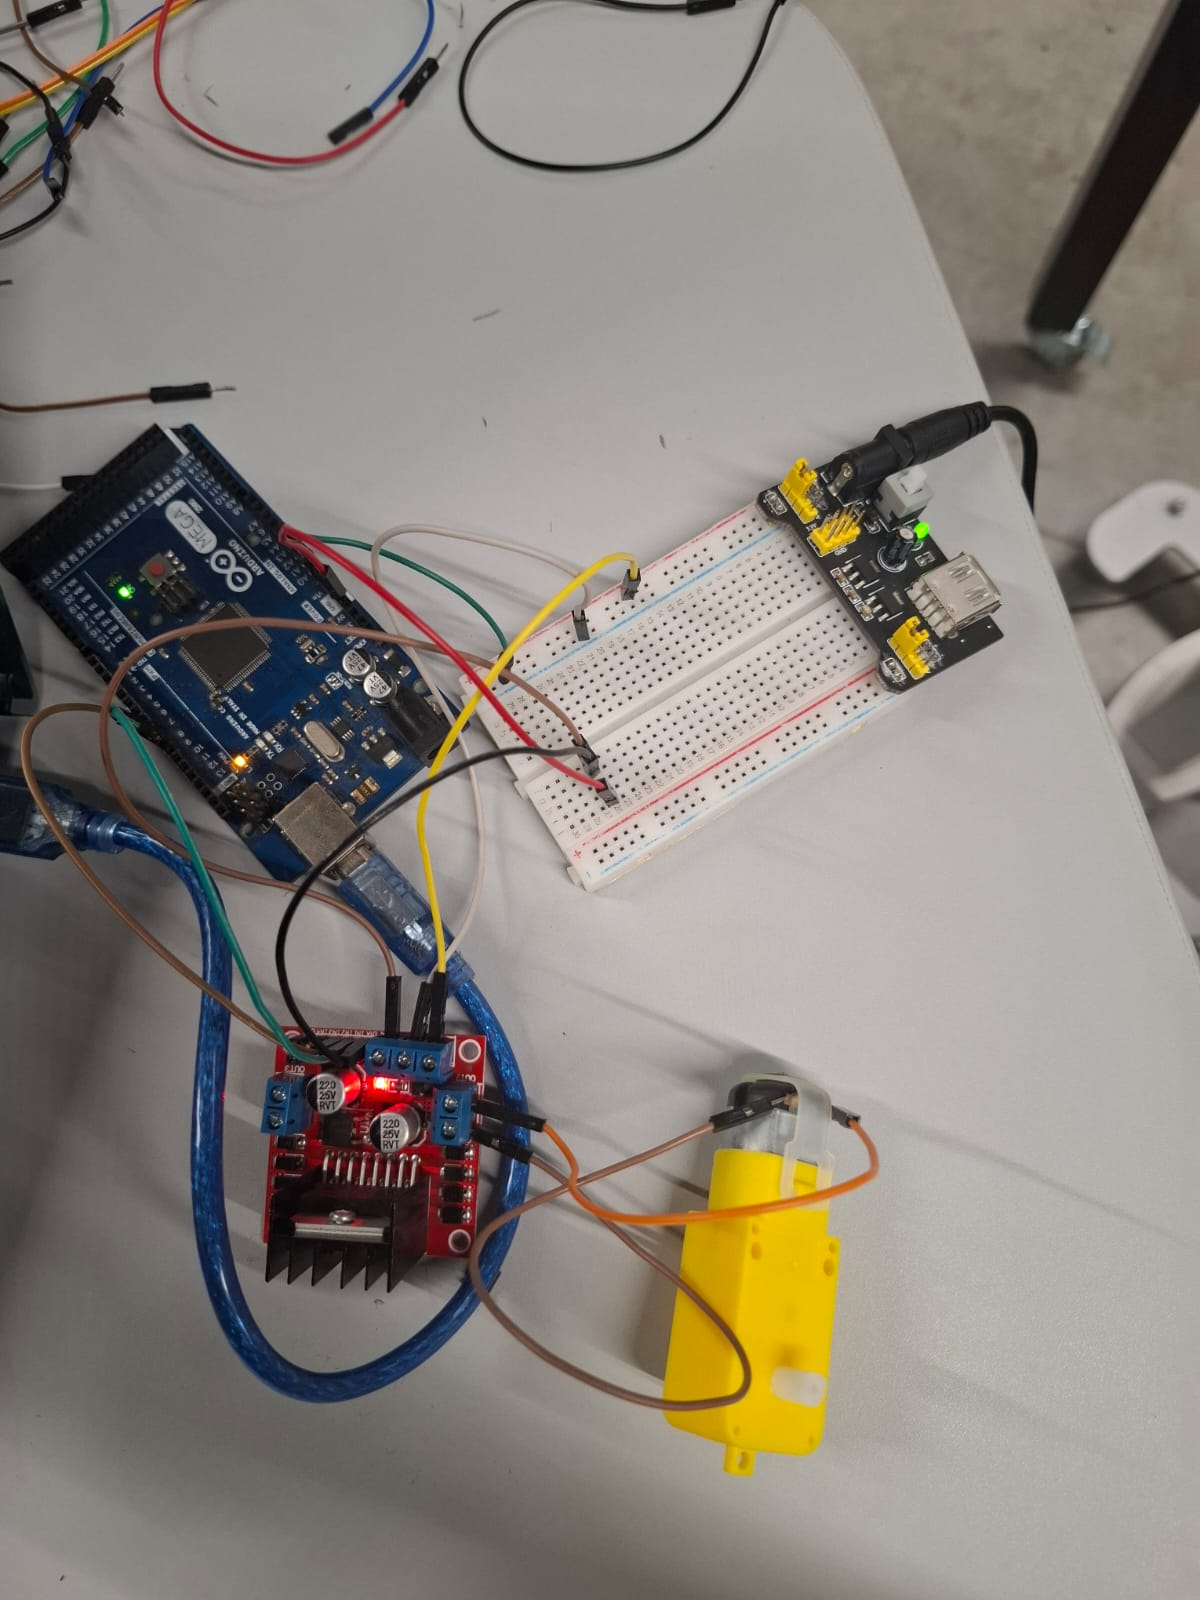
\includegraphics[width=0.85\textwidth]{./img/ckpt_presencial_298.jpeg}
    \caption{Implementación del L298N con Motor}
    \label{fig:motor_driver}
\end{figure}

\begin{figure}[H]
    \centering
    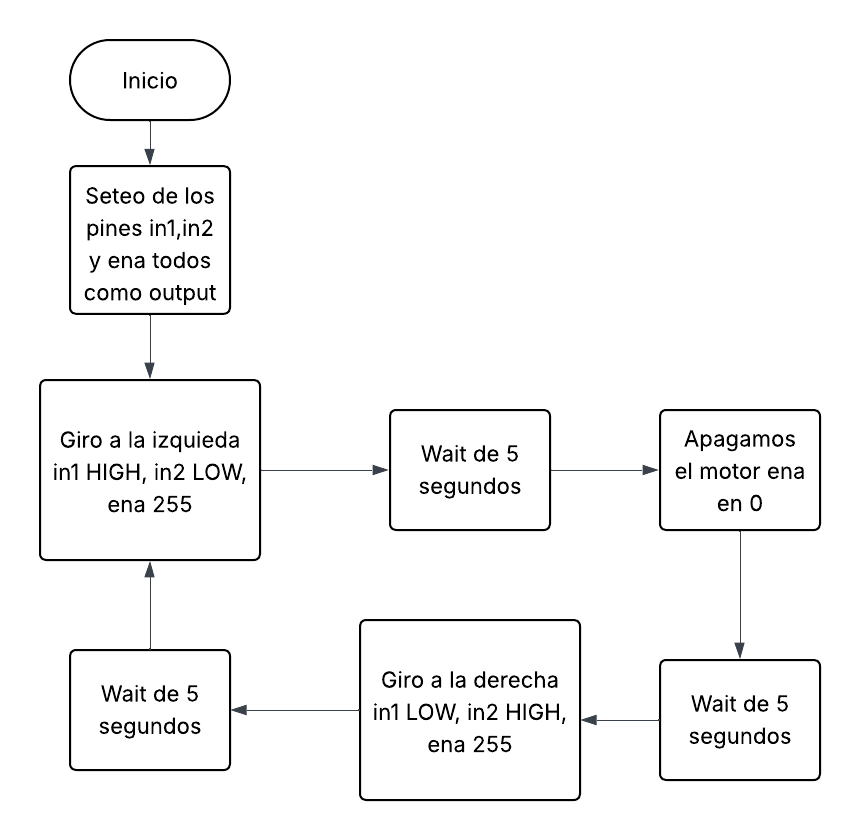
\includegraphics[width=0.85\textwidth]{./img/flujo_298.png}
    \caption{Diagrama de flujo}
    \label{fig:motor_driver}
\end{figure}

% DONE: implementacion
% DONE: respuesta a las preguntas
% DONE: diagrama de flujo
% TODO: diagrama de bloques


\subsection{ACTUADORES - Sistema de riego inteligente}

% TODO: foto de la implementacion presencial en el laboratorio
% TODO: diagrama de flujo
% TODO: diagrama de bloques


\subsection{ACTUADORES - Control de ventiladores}

% TODO: solo simulacion Tinkercad
% TODO: diagrama de bloques del sistema


\section{Conclusiones}

\bibliographystyle{plain}
\bibliography{bibliografia}

\end{document}

\bibliographystyle{plain}
\bibliography{bibliografia}
